\documentclass[brazilian, 12pt, a4paper, final]{article}
\usepackage[utf8]{inputenc}
\usepackage[brazil]{babel}
\usepackage[T1]{fontenc}
\usepackage{multicol}
\usepackage{graphicx}
\usepackage{indentfirst}
\usepackage{amsmath}
\usepackage{array}
\usepackage{caption}
\usepackage[left=1.5cm, right=1.5cm]{geometry}

\title{\textbf{Prova 3}}

\author{Cristiane de Paula Oliveira\\\\\small{Instituto de Física -- Universidade Federal do Rio Grande do Sul}}

\begin{document}

\maketitle

\section*{Questão 1}
\subsection*{1. (a)}
Para que a densidade de probabilidade $\rho(x)$ esteja corretamente normalizada no intervalo é necessário que a integral de $\rho(x)$ no intervalo $[-L,L]$ seja  igual a 1.
Portanto, precisamos calcular
\begin{equation}
	\frac{1}{A}=\int_{-L}^{L}\cos\left(\frac{\pi x}{2L}\right)dx.
\end{equation}
\begin{equation*}
	\frac{1}{A}=\int_{-L}^{L}\cos\left(\frac{\pi x}{2L}\right)dx=\frac{2L}{\pi}\sin\left(\frac{\pi x}{2L}\right)\bigg\rvert_{-L}^{L}=\frac{2L}{\pi}\left(\sin\frac{\pi}{2}+\sin\frac{\pi}{2}\right)=\frac{4L}{\pi}.
\end{equation*}
Assim, 
\begin{equation}
A=\frac{\pi}{4L}.
\end{equation}

\subsection*{1. (b)}
O método da transformada inversa consiste em calcular a função cumulativa $fdc(x)$, cujo valor está no intervalo $[0,1]$, definida como
\begin{equation}
	fdc(	x)=\int_{x_0}^{x}\rho(x')dx'.
\end{equation}
Como $fdc(x)$ possui valores entre 0 e 1, podemos gerar números aleatórios $r$ que correspondem a $fdc(x)$ para determinado $x$. Assim, fazendo a transformada inversa geramos números aleatórios $x$ a partir de $r$ de acordo com a distribuição de probabilidade $\rho(x)$. 

Neste problema,
\begin{equation*}
	r=\frac{\pi}{4L}\int_{-L}^{x}\cos\left(\frac{\pi x'}{2L}\right)dx'=\frac{\pi}{4L}\frac{2L}{\pi}\sin\left(\frac{\pi x'}{2L}\right)\bigg\rvert_{-L}^{x}=\frac{1}{2}\left[\sin\left(\frac{\pi x}{2L}\right)+1 \right].
\end{equation*}

\begin{equation*}
	\sin\left(\frac{\pi x}{2L}\right)=2r-1\Rightarrow x=\frac{2L}{\pi}\arcsin(2r-1).
\end{equation*}
	
\subsection*{1. (c)}
Usando $L=5$ e 100 bins, gera-se o gráfico da figura 1 para diversos valores de $N$.

\begin{figure}[htbp]
  \centering
  \includegraphics[width=0.5\textwidth,angle=-90]{Q1/HistQ1.eps}
  \caption{Histograma para diversos valor de $N$.}
\end{figure}

Para normalizar o histograma, calcula-se a área total do histograma, dada por
\begin{equation}
	Area=\sum_{i=1}^{N}hist[i]\Delta x,
\end{equation} 
e em seguida divide-se cada frequência em $hist[i]$ pela área.

Na figura 2 mostra-se o histograma normalizado.

\begin{figure}[htbp]
  \centering
  \includegraphics[width=0.5\textwidth,angle=-90]{Q1/NormQ1.eps}
  \caption{Histograma normalizado para diversos valores de $N$ e função densidade de probabilizade $\rho(x)$.}
\end{figure}

Percebe-se que os números gerados pelo programa de fato obedecem a distribuição de probabilidade e tendem a se aproximar cada vez mais para $N$ maiores.

%\subsection*{1. (d)}

\section*{Questão 2}
\subsection*{2. (a)}
A solução analítica da integral é
\begin{equation*}
	I=3\int_{-5}^{5} 1-\frac{x^2}{25} dx=3\left[x-\frac{x^3}{75}\right]\bigg\rvert_{-5}^{5}=3\left[10-\frac{10}{3}\right]=20.
\end{equation*}

\subsection*{2. (b)}
\begin{figure}[htbp]
  \centering
  \includegraphics[width=0.5\textwidth,angle=-90]{Q2/IQ2.eps}
  \caption{Integral utilizando (i) tentativa e erro, (ii) estimativa por amostragem simples e (iii) por amostragem por importância.}
\end{figure}

\subsection*{2. (c)}
Na figura 4 são mostrados os valores da integral encontrados pelas três abordagens para diferentes valores de N. Pela figura é possível perceber que o método (ii) se aproxima mais rapidamente do valor exato que o método (i) e o método (iii) ainda mais rapidamente que o método (ii).

O método (i), método da tentativa e erro, consiste em gerar um retângulo de lados $x_{max}-x_{min}$ e $y_{max}=-y_{min}$, onde $x_{min}$ é o início do intervalo em que busca-se calcular a integral, $x_{max}$ é o final, $y_{max}$ é o valor máximo no intervalo  da $f(x)$ e $y_{min}=0$. 

São gerados $N$ pares $(x,y)$ no retângulo e contabiliza-se os número de pares que estão abaixo de $f(x)$. Assim, a integral encontrada a partir dessa abordagem é dada por

\begin{equation}
	I=\frac{S}{N}[(x_{max}-x_{min})-(y_{max}-y_{min})].
\end{equation}

No método (ii), estimativa por amostragem simples, busca-se encontrar o valor médio da função $f(x)$ no intervalo. O valor médio de $f(x)$ pode ser encontrado gerando-se $N$ valores aleatório $x_i$ e calculando-se a média
\begin{equation}
	\mu_N=\frac{1}{N}\sum_{i=1}^{N}f(x_i). 
\end{equation}
Com $\mu_N$, calcula-se então a integral 
\begin{equation}
	I=(x_{max}-x_{min})\mu_N.
\end{equation}

Existem casos em que é preferível que alguns valores de $x$ sejam evitados pois caso contrário podem induzir a erros no cálculo da integral. No método (iii), estimativa por amostragem por importância, os números aleatórios $x_i$ não são gerados uniformemente, e sim, gerados a partir de uma distribuição de probabilidades. 

Sendo assim, a  integral é calculada por
\begin{equation}
	I=\frac{1}{N}\sum_{i=1}^{N}\frac{f(x_i)}{p(x_i)}.
\end{equation}
 
\subsection*{2. (d)}
Por se tratar de um processo estatístico, e não determinístico, o método de Monte Carlo possui flutuações nos valores encontrados a cada repetição. Para verifica se os valores encontrados são coerentes com o esperado, é necessário realizar diversas repetições para verificar se os valores são distribuidos em torno de um valor médio. Geralmente, essa distribuição é a distribuição normal e é possível estimar-se um valor médio e um erro associado.

\section*{Questão 3}
\subsection*{3. (a)}
\begin{figure}[htbp]
  \centering
  \includegraphics[width=0.5\textwidth,angle=-90]{Q3/histQ3.eps}
  \caption{Histogramas da distribuição espacial após 100, 1000 e 1000 passos.}
\end{figure} 

\subsection*{3. (b)}

\begin{figure}[htbp]
  \centering
  \includegraphics[width=0.5\textwidth,angle=-90]{Q3/log100.eps}
  \caption{Histograma com ajuste da função $f(x)=bx^2+log(a)$ para 100 passos.}
\end{figure} 

\begin{figure}[htbp]
  \centering
  \includegraphics[width=0.5\textwidth,angle=-90]{Q3/log1000.eps}
  \caption{Histograma com ajuste da função $f(x)=bx^2+log(a)$ para 1000 passos.}
\end{figure}      
  
\begin{figure}[htbp]
  \centering
  \includegraphics[width=0.5\textwidth,angle=-90]{Q3/log10000.eps}
  \caption{Histograma com ajuste da função $f(x)=bx^2+\log(a)$ para 10000 passos.}
\end{figure} 

	\begin{table}[hptb]
    \centering
    \begin{tabular}{c|c|c}
	 Passos  	&	a	&	b	 \\ 
    \hline
    $100$	&	$7622.3\pm459.9$	&	$-0.0049082\pm7.299e-05$\\ 
    $1000$	&	$2332.78\pm81.13$	&	$-0.000476007\pm4.671e-06$\\ 
    $10000$	&	$718.037\pm20.08$	&	$-4.69867e-05\pm4.241e-07$\\ 
    \end{tabular}
    \caption{Parâmetros dos ajustes da função $f(x)=bx^2+\log(a)$ aos logaritmos dos histogramas.}
\end{table}
	
%\subsection*{3. (c)}

%\subsection*{3. (d)}

%\subsection*{3. (e)}

%\section*{Questão 4}
%\subsection*{4. (a)}

%\subsection*{4. (b)}
	
%\subsection*{4. (c)}

%\subsection*{4. (d)}

%\subsection*{4. (e)}

\section*{Questão 5}

\begin{figure}[htbp]
  \centering
  \includegraphics[width=0.5\textwidth,angle=-90]{Q5/VarQ5.eps}
  \caption{Variância da integral para diferentes $a$. Ajusta-se uma parábola para encontrar o valor de $a$ que minimiza a variância. Encontra-se que $a\approx0,55$ é o que minimiza a variância.}
\end{figure} 

\begin{figure}[htbp]
  \centering
  \includegraphics[width=0.5\textwidth,angle=-90]{Q5/Q5comp.eps}
  \caption{Estimativa da integral em 100 repetições utilizando o método da amostragem por importância e amostragem uniforme.}
\end{figure} 

Pela figura 9, percebe-se que o método da amostragem por importância tende a ter uma dispersão muito menor em torno do valor real da integral do que o método da amostragem uniforme. Isso se deve pois o método da amostragem por importância calcula a integral utilizando valores $x$ aleatórios a partir de uma distribuição de probabilidade, dando peso maior para valores de $x$ que mais contribuem para que a estimativa da integral seja mais próxima do valor real.
%\section*{Questão 6}

\end{document}

